\documentclass[11pt, oneside]{article}   	% use "amsart" instead of "article" for AMSLaTeX format
\usepackage{geometry}                		% See geometry.pdf to learn the layout options. There are lots.
\geometry{letterpaper}                   		% ... or a4paper or a5paper or ... 
%\geometry{landscape}                		% Activate for rotated page geometry
\usepackage{graphicx}				% Use pdf, png, jpg, or eps§ with pdflatex; use eps in DVI mode
								% TeX will automatically convert eps --> pdf in pdflatex
\usepackage{url}
\usepackage{amssymb}
\usepackage{listings}
\usepackage{amsmath}
\usepackage[utf8]{inputenc} 
\usepackage[export]{adjustbox}
\usepackage{siunitx}

%begin documents

\title{Unit Testing}
\author{Alexander Dean}
%\date{}					% Activate to display a given date or no date

\begin{document}
\maketitle
\section{Introduction}
When programming the notion of testing is used to understand if there are any errors in code. It can catch errors such as syntax errors, assertion errors, name errors, \dots However, we can also test that a process has worked as expected, for example in predictive modelling, we can test that the distribution of predictions matches our prior beliefs. It can be a daunting task to test a whole script, therefore it makes sense to test code in units and this practice is termed unit testing. It is often required that the units are easily identifiable, perhaps the code is written in classes and functions, where each of the units are independent from each other. In a development environment we create a separate tests folder containing separate test scripts for the code that is being tested. Some key terminology similar to \cite{WEBSITE:3} is given as:

\begin{enumerate}
\item Test step - Define a test to be run (e.g turning the headlights on in a car)
\item Test assertion - What outcomes are we expecting (e.g check if the headlights are on)
\item Test case - Combination of a test step and assertion
\item Test framework - This is a platform that has all the tools and libraries organised and set in a structure to enable automation testing. An analogy can be made to a train station, a train stations set up (platform, ticket counter, trains, ticket office, ...) have a structure that make it very easy to catch a train \cite{WEBSITE:1}
\item A test runner - Sets up the execution of tests and provides the outcome to the user.
\end{enumerate}

\section{Writing unit tests}
We will explore testing in python using the unittest module. All unit test scripts need to be saved with filename according to the convention test\_*.py, this will enable a clear project structure and running of tests. Lets say we create a script even\_check.py that contains a function to test if a number is even. A similar process is given in \cite{WEBSITE:2}\\

\begin{lstlisting}[language = python]
#check if a number is even
def is_even(number):
    #is the modulus after dividing by 2 zero?
    if number%2 ==0:
        return 1
    else:
        return 0
        
\end{lstlisting}

W now test the is\_even function by creating a file test\_even\_check.py with the following test.
\\
\begin{lstlisting}[language = python]
#testing the is_even function 
import unittest
from even_check import is_even
#create a class that inherits from the TestCase class
class EvensTestCase(unittest.TestCase):
    """Tests for even_check.py"""
    #convert functions to methods by passing self as an argument
    def test_is_2_even(self):
        """Is 2 even?"""
        self.assertTrue(is_even(2))

#run the tests when the script is passed through the intepreter
if __name__ == '__main__':
    unittest.main()
    
\end{lstlisting}

This file has created a unit test with a single unit test case; which tests if 2 is even. Of course, since 2 is even,  we would expect this test to run successfully and the results of this test are shown below.

\begin{figure}[h]\label{fig:roc1}
  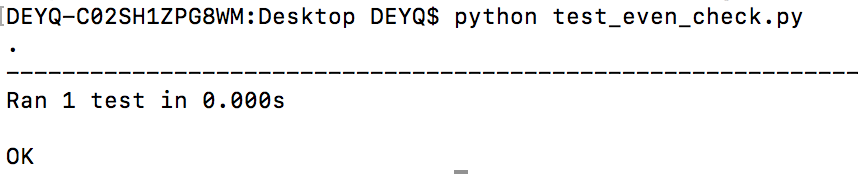
\includegraphics[width=0.5\linewidth,center] {unit_test_results.png}
  \caption{Unit test results}
\end{figure}

We have made use of the package unittest and pythons built in unit test framework. We can explain the detail contained in the test\_even\_check.py file. Any member function in a class derived from unittest.TestCase and whose name begins test will be run, when unittest.main() is called. Note when a python interpreter reads a source file it does an important step, it sets variables like\_\_name\_\_. In fact,  when the interpreter reads the script, it assigns the hard coded string "\_\_main\_\_" to the \_\_name\_\_ variable. Note an interpreter is an application which will  run the python script. So clearly, in our test script we will be invoking the unititest.main() method. This method triggers other methods within unittest, one of which is runTests. So the last few lines of code are instructions to run the tests that we have defined within the script test\_even\_check.py, when the program is ran through a python interpreter. In our script above we have made use of unittest's assert true method which asserts that the argument passed to it is true. There are a wide range of other asset methods available listed in \cite{WEBSITE:4}.

\section{Principles of unit testing}

There are some key guidelines for how unit tests should be carried out in the F.I.R.S.T framework as shown in \cite{WEBSITE:5}.
\begin{enumerate}
\item Fast - tests should run quickly
\item Isolated/Independent - The order tests are run should not matter, the assert should test only a single logical outcome
\item Repeatable - A test method should not depend on any data in the instance that it is running, each test should set up or arrange its own data
\item Self-Validating - No manual inspection required to check whether the test has passed or failed
\item Thorough - Should cover most cases 
\end{enumerate}

\newpage
\bibliography{/Users/DEYQ/Desktop/unit_testing/sources}
\bibliographystyle{plain}

\end{document}